\documentclass[12pt]{article}

\usepackage[english,serbian]{babel}
\usepackage{graphicx}
\usepackage{caption}
\usepackage{url}

\title{African Soil Property Prediciton}
\author{Ognjen Sretenović, Katarina Jokanović}

\begin{document}

\maketitle

\twocolumn

\section{Uvod}
Kako bi planiranje izdržive agrikulturalne infrastrukture bilo moguće na mestima o kojima imamo malo podataka, kao što je Afrika, veliki značaj pokazuje digitalno mapiranje funkcionalnih karakteristika zemljišta, kao što su otpornost na eroziju i sadržaj vode i hranljivih materija.

Kao potencijalno značajan, brz i jeftin metod merenja ovih karakteristika pokazuje se \textit{difuzna infracrvena spectroskopija}, kojom se meri interakcija infracrfvene radijacije sa materijom, u našem slučaju sa uzorcima zemljišta.

\subsection{Podaci}
Data set čine podaci o reprezentativnim uzorcima zemljišta sa površine od oko 18 miliona kvadratnih kilometara nepustinjskih delova Afrike i Madagaskara, sakupljanih u okviru \textit{Africa Soil Information Service} projekta.

Uzorci su podeljeni u dve grupe na osnovu dubine - Topsoil (0cm-20cm) i Subsoil (20cm-50cm), i svakom uzorku je dodeljen identifikator.

Imamo 3578 mera apsorpcije na talasnim dužinama u opsegu od$~1.3\mu m$ do$~16.6 \mu m$.

Pored toga, imamo prosečne dugoročne podatke o tropskim padavinama (TMAP, TMFI) i složeni topografski index (CTI).

Od podataka sa \textit{Shuttle Radar Topography} misija imamo podatke o nadmorskoj visini (ELEV) i topografskom reljefu (Reli).

Sa MODIS satelitskih slika imamo dugoročna merenja površinske temperature (LST), prosečna dugoročna \textit{Black-Sky Albedo} merenja (BSA) i prosečna dugoročna merenja refleksije (Ref). 

\subsection{Izlazna obeležja}
Ovim podacima želimo da predvidimo sledeća svojstva zemljišta:
\begin{itemize}
	\item Ca - Mehlich-3 sxtractable Calcium
	\item P - Mehlich-3 extractable Phosphorus
	\item pH - pH vrednosti
	\item SOC - Soil organic carbon
	\item Sand - sadržaj peska
\end{itemize}

\section{Priprema podataka}
Iz podataka za treniranje smo izbacili obeležje \textit{PIDN} koje predstavlja identifikator uzorka.

Obeležje \textit{Depth} smo mapirali na numeričke vrednosti (Topsoil $\rightarrow$ 0, Subsoil $\rightarrow$ 1).

\subsection{Outlier-i}
Jedna od stvari koje smo pokušali jeste izbacivanje outlier-a, međutim time smo gubili skoro trećinu podataka, pa smo odlučili da ograničimo podatke na minimum (vrednost prvog kvartila - 1.5 * interkvartilni opseg) maksimum (vrednost trećeg kvartila + 1.5 * interkvartilni opseg). Ovo nije uticalo na performanse modela.

\subsection{Visoko korelisani podaci}
Kako za svaki uzorak imamo 3578 vrednosti apsorpcije po različitim talasnim dužinama očekivali smo da su one u određenoj meri korelisane, što bi uticalo na performanse modela, pa smo odlučili da izbacimo iz data seta podatke sa korelacijom iznad 95\%, što nas je ostavilo sa 19 kolona.

Performanse modela nakon ovoga su se uglavnom poboljšale, osim za \textit{KNearestNeighbours} algoritam koji je bez korelisanih kolona dao lošije rezultate.

\subsection{Polynomial Features}
Svaki algoritam smo trenirali i uz \textit{Polynomial Features} drugog stepena kako bi videli da li kombinacijama atributa možemo pronaći dodatne zakonitosti.

Takođe, ovo smo radili samo nakon izbacivanja korelisanih podataka.\footnote{Zanimljiva činjenica: \textit{polynomial features} drugog stepena kreirao je 6463810 kolona koje bi zauzele 35.6GB RAM memorije, malo više od onoga što imamo pri ruci}

\subsection{Feature Selection}
Za dva algoritma, linearnu regresiju koja se pokazala najgore i KNN koji se pokazao najbolje, smo upotrebili i Forward i Backward sekvencijalnu selekciju atributa, što je u oba slučaja dalo lošije rezultate.

\section{Algoritmi}
\subsection{Ocena}
Za ocenjivanje regresionih modela koristili smo \textit{Mean Columnwise Root Mean Squared Error}
$$MCRMSE = \frac{1}{5}\sum_{j=1}^{5}\sqrt{\frac{1}{n}\sum_{i=1}^{n}(y_{ij}-\hat{y_{ij}})^2}$$
odnosno prosek korene srednje kvadratne greške po svojstvima koje pre\-dviđamo.

\subsection{Trening}
Svaki model smo trenirali kroz \textit{Grid Search} kros validaciju sa RMSE kriterijumom.

Data set smo podelili na \textit{trening set} (80\%) i \textit{test set} (20\%).

\onecolumn

\subsection{Modeli}
Modeli trenirani algoritmom \textbf{linearne regresije} su se pokazali najgore u svim slučajevima.

Modeli trenirani algoritmom \textbf{regresionog stabla} su bili bolji.

\textbf{Random forest} algoritmom trenirali smo dva modela, bez korelisanih obeležja sa i bez \textit{polynomial features}-a i njihovi rezultati su blizu najboljim koje smo dobili.

Algoritam \textbf{k najbližih suseda - KNN} dao nam je najbolje modele. Takođe, najbolji rezultat je dao na data setu pre izbacivanja visoko korelisanih obeležja.

\begin{table}[!ht]
    \centering
    \begin{tabular}{|l|l|l|l|l|l|l|}
    \hline
        model & Ca & P & pH & SOC & Sand & MCRMSE \\ \hline
        lin\_reg & 0.505 & 1.658 & 0.754 & 0.705 & 0.729 & 0.87 \\ \hline
        tree & 0.565 & 1.059 & 0.675 & 0.53 & 0.524 & 0.671 \\ \hline
		\textbf{knn} & 0.371 & 0.755 & 0.537 & 0.464 & 0.453 & \textbf{0.516} \\ \hline
        lin\_reg\_clipped & 0.505 & 1.658 & 0.754 & 0.705 & 0.729 & 0.87 \\ \hline
        tree\_clipped & 0.565 & 1.059 & 0.675 & 0.53 & 0.524 & 0.671 \\ \hline
        knn\_clipped & 0.371 & 0.755 & 0.537 & 0.464 & 0.453 & 0.516 \\ \hline
        lin\_reg\_bez\_korelacija & 0.833 & 0.699 & 0.68 & 0.832 & 0.77 & 0.763 \\ \hline
        tree\_bez\_korelacija & 0.511 & 0.725 & 0.616 & 0.723 & 0.526 & 0.62 \\ \hline
        knn\_bez\_korelacija & 0.679 & 0.764 & 0.568 & 0.629 & 0.544 & 0.637 \\ \hline
        random\_forest\_bez\_korelacija & 0.516 & 0.866 & 0.508 & 0.559 & 0.419 & 0.573 \\ \hline
        lin\_reg\_bez\_korelacija\_pol & 0.642 & 0.699 & 0.619 & 0.766 & 0.671 & 0.679 \\ \hline
        tree\_bez\_korelacija\_pol & 0.511 & 0.725 & 0.616 & 0.723 & 0.526 & 0.62 \\ \hline
        knn\_bez\_korelacija\_pol & 0.679 & 0.764 & 0.568 & 0.629 & 0.544 & 0.637 \\ \hline
        random\_forest\_bez\_korelacija\_pol & 0.528 & 0.922 & 0.504 & 0.567 & 0.416 & 0.588 \\ \hline
        lin\_reg\_bez\_korelacija\_selection & 0.828 & 0.692 & 0.682 & 0.858 & 0.801 & 0.772 \\ \hline
        knn\_bez\_korelacija\_selection & 0.582 & 0.687 & 0.537 & 0.605 & 0.413 & 0.565 \\ \hline
    \end{tabular}
\end{table}

\captionof{table}{Ocene modela po izlaznim obeležjima}

\pagebreak

\section{Primena modela}
Nakon treninga svakog modela na ranije pomenuti način izdvojali smo parametre sa kojima model daje najbolje rezultate i sa njima ponavljali trening, ovaj put na celom data setu.

Ovako trenirane finalne modele koristili smo za predviđanje na osnovu podataka iz \textit{sorted\_test} data seta i rezultate predavali na kaggle.

Ocena prvog modela linearne regresije koji smo kreirali bila je 1.08, a ocena najboljeg KNN modela 0.74.

\begin{figure}[!h]
\centering
  
\includegraphics[width=0.9\columnwidth]{photos/results1.jpg}
  \caption{kaggle score - linearna regresija}
\end{figure}

\begin{figure}[!h]
\centering
  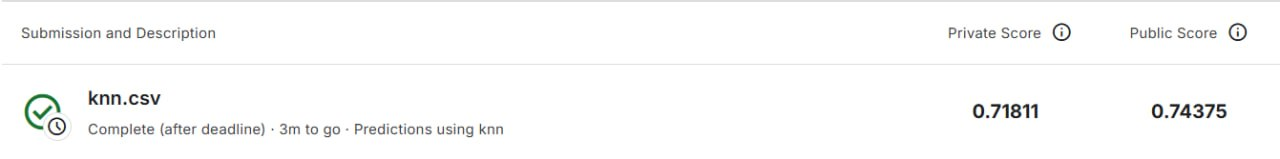
\includegraphics[width=0.9\columnwidth]{photos/results2.jpg}
  \caption{kaggle score - knn}
\end{figure}

\section{Zaključak i budući pravci}
Na kraju se osećamo malo nezadovoljno činjenicom da se nakon svog truda najbolje pokazao običan KNN.

Žao nam je i što zbog hardware-skih ograničenja nismo mogli da treniramo modele primenom \textit{Boosting} algoritama, treniramo Random Forest model i primenimo \textit{Sequential Feature Selection} na data setu pre izbacivanja visoko korelisanih kolona.

\pagebreak
\twocolumn
	\footnotesize
\nocite{*}
\bibliographystyle{plain}
\bibliography{literatura}


\end{document}
